% THIS IS SIGPROC-SP.TEX - VERSION 3.1
% WORKS WITH V3.2SP OF ACM_PROC_ARTICLE-SP.CLS
% APRIL 2009
%
% It is an example file showing how to use the 'acm_proc_article-sp.cls' V3.2SP
% LaTeX2e document class file for Conference Proceedings submissions.
% ----------------------------------------------------------------------------------------------------------------
% This .tex file (and associated .cls V3.2SP) *DOES NOT* produce:
%       1) The Permission Statement
%       2) The Conference (location) Info information
%       3) The Copyright Line with ACM data
%       4) Page numbering
% ---------------------------------------------------------------------------------------------------------------
% It is an example which *does* use the .bib file (from which the .bbl file
% is produced).
% REMEMBER HOWEVER: After having produced the .bbl file,
% and prior to final submission,
% you need to 'insert'  your .bbl file into your source .tex file so as to provide
% ONE 'self-contained' source file.
%
% Questions regarding SIGS should be sent to
% Adrienne Griscti ---> griscti@acm.org
%
% Questions/suggestions regarding the guidelines, .tex and .cls files, etc. to
% Gerald Murray ---> murray@hq.acm.org
%
% For tracking purposes - this is V3.1SP - APRIL 2009
\documentclass{acm_proc_article-sp}

\usepackage{url}
\usepackage{listings}
\usepackage{algpseudocode}
\usepackage{graphicx}
\DeclareGraphicsExtensions{.pdf,.png}

\begin{document}

\title{Side-effect disparity as a metric for identifying behavioral subtyping violations}
\subtitle{[COM S 610 --- Fall 2013 --- Final project report]}
%
% You need the command \numberofauthors to handle the 'placement
% and alignment' of the authors beneath the title.
%
% For aesthetic reasons, we recommend 'three authors at a time'
% i.e. three 'name/affiliation blocks' be placed beneath the title.
%
% NOTE: You are NOT restricted in how many 'rows' of
% "name/affiliations" may appear. We just ask that you restrict
% the number of 'columns' to three.
%
% Because of the available 'opening page real-estate'
% we ask you to refrain from putting more than six authors
% (two rows with three columns) beneath the article title.
% More than six makes the first-page appear very cluttered indeed.
%
% Use the \alignauthor commands to handle the names
% and affiliations for an 'aesthetic maximum' of six authors.
% Add names, affiliations, addresses for
% the seventh etc. author(s) as the argument for the
% \additionalauthors command.
% These 'additional authors' will be output/set for you
% without further effort on your part as the last section in
% the body of your article BEFORE References or any Appendices.

\numberofauthors{1} %  in this sample file, there are a *total*
% of EIGHT authors. SIX appear on the 'first-page' (for formatting
% reasons) and the remaining two appear in the \additionalauthors section.
%
\author{
% You can go ahead and credit any number of authors here,
% e.g. one 'row of three' or two rows (consisting of one row of three
% and a second row of one, two or three).
%
% The command \alignauthor (no curly braces needed) should
% precede each author name, affiliation/snail-mail address and
% e-mail address. Additionally, tag each line of
% affiliation/address with \affaddr, and tag the
% e-mail address with \email.
%
% 1st. author
\alignauthor
Lor\'{a}nd Szak\'{a}cs\\
       \affaddr{Iowa State University}\\
       \email{lorand@iastate.edu}
% 2nd. author
}
% There's nothing stopping you putting the seventh, eighth, etc.
% author on the opening page (as the 'third row') but we ask,
% for aesthetic reasons that you place these 'additional authors'
% in the \additional authors block, viz.
% Just remember to make sure that the TOTAL number of authors
% is the number that will appear on the first page PLUS the
% number that will appear in the \additionalauthors section.

\maketitle

\abstract
When dealing with class hierarchies in object oriented languages programmers are faced with the problem of verifying that subtypes respect the contracts of their supertypes. Formal specification solves this, but it suffers from the caveat that specification has to be written in addition to code. This paper proposes an alternative, light-weight heuristic for detecting behavioral subtyping violations by looking solely at the side-effects of the code. We have evaluated this heuristic against a very large corpus of code and we have concluded that it has the potential of being applicable in practice. 

\section{Introduction}\label{section:intro}
Behavioral subtyping (\emph{a.k.a.} \emph{Liskov Substitution Principle}) is an object oriented heuristic that aims to make a distinction between extension and subtyping, whereas extension means that the subclass simply inherits implementation and instantiations of it are assignable to references of its superclass' with no guarantee that at runtime it will behave as expected. While subtyping implies guarantees that when instantiations of the subclass are used, they behave as expected allowing for programmers to reason in terms of what is called supertype abstraction~\cite{leavens1995specification}. An essentially equivalent definition of behavioral subtyping is given by~\cite{america1991designing, liskov1994behavioral, liskov1999behavioral, meyer1988object}: subtypes are allowed to weaken the pre-conditions and strengthen the post-conditions imposed by their supertypes.

The \emph{Liskov Substitution Principle} is regarded as a corner stone guideline in object oriented design, being part of the so called SOLID principles~\cite{martin2000design, martin2003agile}. This idea has been part of the zeitgeist of industry programmers since at least 1988~\cite{meyer1988object} and has been brought forward as a good guideline by famous speakers like Robert C. Martin and Bertrand Meyer. Therefore the importance of this practice cannot be ignored and the need to create automated support to help programmers follow this practice is also a good idea. 

The research community has described behavioral subtyping in terms of formal specification~\cite{america1991designing, liskov1994behavioral, liskov1999behavioral}. Which has its disadvantages, chiefly as the fact that formal specification has to be written separately from, and in a different language than the source code. Therefore testing for behavioral subtyping violations in terms of specification~\cite{duncan1998adding, leavens2006jml, karaorman1999jcontractor, findler2001behavioral} might not be an option at all. 

We offer an alternative way of testing whether or not behavioral subtyping is violated by defining a heuristic in terms of side-effects, more precisely, the disparity between the side-effects of a method in a supertype and the side-effects of its overridden version in any of its subtypes.
We test this heuristic using the Boa language~\cite{dyer2013boa:icse, dyer2013boa:gpce} by collecting data from 5113 open source Java projects. We use these initial empirical results to suggest improvements on the heuristic presented below. Furthermore, the collected data serves as a baseline for comparison of future results obtained with an improved heuristic.

\subsection{Heuristic}
Looking at the side effects of a method might not be enough to infer its behavior, but given the fact that we want to look at the difference in behavior we think that looking at the difference in the side-effects of methods is a good starting point.  This heuristic has the advantage of being simple, both in terms of the complexity of its definition and in terms of relative ease with which it can be automatically applied to code. Essentially, this heuristic allows the inference of and ad-hoc specification for a method purely in terms of its side-effects. Disadvantages are discussed in detail in section~\ref{section:threats}.

\subsection{Related work}
There exist numerous tools and approaches that rely on formal specification to test for behavioral subtyping violations, or as it is referred to in literature behavioral contract violations \cite{duncan1998adding, gomes1996language, karaorman1999jcontractor, kramer1998icontract, plosch1999contracts}. These approaches have the obvious limitation that a code specification \emph{has} to be written. Our approach, on the other hand, relies solely on the source code, therefore making it universally applicable. However, unlike the above mentioned work, our approach cannot be applied to verifying behavioral contract violations by implementors of interfaces and abstract methods. Neither does it concern itself with the actual values of object state, which formal specification tools do.

To the author's knowledge no work exists that uses side-effect disparity between supertype-subtype method effects to test for behavioral subtype violations.
\section{Approach}
This study seeks to answer two research questions: \emph{(RQ1) is side-effect disparity a valid heuristic for identifying behavioral subtyping violations?} And, a secondary, less substantiated research question whose answer depends on the answer of the first research question: \emph{(RQ2) to what extent does behavioral subtyping happen in practice?}

To address these questions we took the following high level approach:
\begin{itemize}
\item define a heuristic for identifying behavioral subtyping violations
\item use Boa to apply this heuristic to a large number of real world projects (this answers \emph{RQ2})
\item manually inspect several violations to determine whether or not the identification was accurate (this  answers \emph{RQ1})
\item based on results, suggest improvements
\end{itemize}

\subsection{Definition of side-effects}\label{definition:side-effects}
For the purposes of this study we looked at a restricted definition of side-effects. We included only:
\begin{itemize}
\item assignments to the fields of a class, includes inherited fields
\item method calls on fields of the class
\item calls to methods from the class in question
\end{itemize}
For instance, consider the following contrived example:
\begin{lstlisting}
  void foo(P param) {
    this.myField = 42;
    super.superField = 24;
    int localVar = this.f1;
    param.field = 42;
    localBar();
    myField.otherBar();
  }
\end{lstlisting}
The effects of this method would be: \emph{myField, superField, localBar() and otherBar().} Methods \emph{localBar()} and \emph{otherBar()} are not substituted for their effects.

\subsection{Side-effect disparity}
Side-effect disparity as a heuristic for determining behavioral subtyping violations is motivated by two arguments:
\begin{enumerate}
\item from Leavens et al~\cite{leavens2006jml, leavens2006design} we can see that in the JML specification language the post conditions of a method are the side-effects of a method. Therefore, if we compute the side effects of a method in a super-class, we can use its side-effects as an inferred post-condition of the superclass method. Therefore, by comparing the side-effects of two methods we are implicitly comparing their post-conditions. And disparities in the post-conditions can imply violations in behavioral subtyping.
\item side-effects are also a reflection of the behavior of a program, although in of themselves they cannot be used to infer any behavior. However, the difference in the side-effects of two methods implies a difference in behavior. The extent to which this difference represents a behavioral subtyping violation is the approximation in this heuristic.
\end{enumerate}

Given that we use this heuristic to determine behavioral subtyping violations, only the effects of overridden and overriding methods need to be computed.

\subsection{Comparison}
In this sub-section we will present a high level overview of the employed analysis.
The Boa implementation and its limitations are further explored in section~\ref{section:implementation}.

The following algorithm operates on an entire project. The results stored in the \emph{violations} collection are aggregated for all projects.
\begin{algorithmic}
\State Input: Project
\State $PBS \gets \Call{gatherAllSubtype-SuperTypePairs}{}$
\ForAll{$classPair$ in $PBS$}
  
  $OM \gets \Call{gatherOverridenMethods}{classPair}$
  
  \ForAll{$(subMethod, superMethod)$ in $OM$}
    \State $subEff \gets \Call{computeSetOfEffects}{subMethod}$

    \State $superEff \gets \Call{computeSetOfEffects}{superMethod}$
    
    \If{$subEff$ - $superEff$ != 0} 
      \State $violations \gets (Project, classPair,$ 
                     \State $subMethod, superMethod)$
    
    \EndIf
  \EndFor

\EndFor
\end{algorithmic}

Very important to note is that when gathering all subtype-supertype pairs we do not account for
transitive inheritance (class \emph{A} extends \emph{B} which extends \emph{C}; so pair \emph{A, C} is never returned). As \cite{america1991designing, szyperski2002component} point out, interface inheritance and implementation inheritance are theoretically two different mechanisms, but in Java they are treated the same therefore the programmer might not intend to subtype the entire family of supertypes, only the explicitly named one.

Another important remark is the fact that we cannot gather subtype-supertype pairs where the supertype is imported from a library or from a project. Thus we do not test \emph{all} subtyping relationships that exists within a project.

The effects of a method are computed as a set of single effects that fit the description given in sub-section~\ref{definition:side-effects}.

\section{Implementation}\label{section:implementation}
The source code of our analysis is available at~\cite{github2013}. It contains all the programs necessary to re-run this analysis as well as a readme file containing all the relevant information to do so. The repository will not be updated after the date of December 13th 2013 so that it reflects the analysis as it was at the time of writing of this report.

The following image describes at a high level the components involved in the implementation of the above pseudo code algorithm:
     
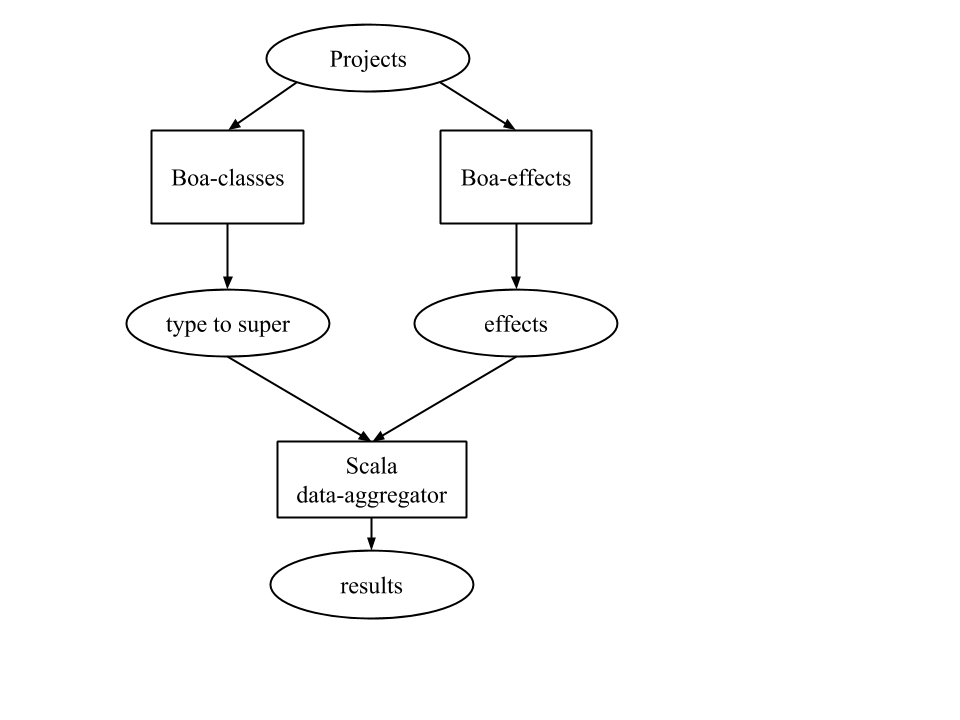
\includegraphics[width=0.5\textwidth, clip=true, trim= 125px 90px 300px 20px]{high-level}

Due to an apparent bug in the runtime of the Boa framework the program had to be divided as above. Otherwise, every computation would have been done in Boa. The program \emph{Boa-classes} outputs a list of all available classes and a list of pairs of classes in a subtype-supertype relationship grouped per project. The program \emph{Boa-effects} program uses the \emph{Boa-classes} as a subroutine to determine all pairs of subtype-supertype and then outputs a list of all the effects of the methods of these classes grouped per method, per class,  per project. This data is then fed to the Scala~\cite{odersky2004overview} program \emph{Scala data-aggregator} which determines the set of pairs of overriden methods, compares their effects and outputs the results. The output is in the form of high level statistics (number of subtype-supertype pairs, etc.) and a file containing a list of \emph{all} behavioral subtyping violations together with the information needed to locate them in the codebase (project id, fully qualified class name, method name).

\subsection{Advantages of Boa}
Boa had three major advantages that greatly work in our favor:
\begin{itemize}
\item easy and convenient access to a very large code base. Cummulatively it took approximately 20 minutes to run the Boa analyses on the 5133 projects, giving us more time to focus on refining the theoretical aspects of this paper.
\item convenient and compact syntax for defining program analysis at an AST node level. This allowed for a relatively simple implementation of side-effect computation by visiting each AST node within a method and retaining only the relevant ones mentioned in section~\cite{definition:side-effects}.
\item reproducibility. The source code of the analyses used to gather the results discussed here can be accessed via~\cite{boa-classes} and~\cite{boa-effects}, the webpages make the output of the analyses downloadable. Then, the \emph{Scala data-aggregator} program has to be run on the downloaded output to produce the results.
\end{itemize}

\subsection{Limitations of Boa}
Boa doesn't offer semantic static analysis data (e.g. fully resolved type information), consequently our analyses had to implement a few features using approximations, and we had to push back others to the future work section (substituting methods with their computed effects). An example sub-routine that had to be written because of the lack of type information is identifying the fully qualified name of the supertype after an \emph{extends} clause. The only information we had about the extended class was its name in string form. So we had to build a fully qualified name based on the following cases and check to see if it is available in a previously computed set containing the fully qualified names of all classes in the project: the actual extended class can be referred to by its fully qualified name, it can be explicitely imported, it can be imported with a wildcard, or it can exist in the same package as its subtype. Determining the fully qualified names of denoted supertypes is sound and complete with respect to the set of classes within the project.

\section{Evaluation}
The Boa framework runs on cached snapshots of the major repository hosting services. When running a Boa program the user is presented with an option to choose on which snapshot to run the analysis. We ran the analysis on the \emph{September 2013 (medium)} snapshot.

\subsection{Results}
Running our analysis on the above snapshot yielded the following results:
\paragraph{RES1}
\emph{1286} of \emph{5133} projects contained at least one class that used implementation inheritance (override a method that already had an implementation). Showing that approximately 25\% of projects use implementation inheritance. Conversely, this shows that 75\% of projects do not use implementation inheritance at all and are, therefore, implicitly using behavioral subtyping. Unfortunately, testing whether or not behavioral subtyping is violated in the case of these 75\% can be done only with the formal specification approach described in the related work section.
\paragraph{RES2}
\emph{739} of these \emph{1286} eligible projects contained at least one subtyping violation.
\paragraph{RES3}
\emph{11600} of \emph{101433} pairs of subtype-supertype contained at least one violation.
\paragraph{RES4} \emph{283216} of \emph{2701596} overridden methods were violating behavioral subtyping.

To answer \emph{RQ1} we have chosen, at random, 4 projects that contained at least one violation, randomly selected 5 violations from each, making for a total of 20 violations; the we tried to determine whether or not they truly constitute behavioral subtyping violations.

 A complete list of the 20 violations, together with each individual verdict is given in section~\ref{ref:data}. In summary, it was determined that \emph{9} out of the \emph{20} violations were false positives. Giving our analysis a precision of 55\%. Given a \emph{correct} specification, the tools mentioned in the related work section have a precision of 100\%. But, also considering (i) the low prevalence of specification, (ii) the room for error in writing the specification, (iii) the fact that our heuristic can be easily applied to any implementation inheritance hierarchy, (iv) the suggestions for improving this heuristic discussed in section~\ref{section:future}; we think that this heuristic can have the potential to be a real alternative to approaches that use formal specification.
 
Given this precision we can now give an answer to \emph{RQ2}: considering results \emph{RES3 and RES4} we can deduce that 6.2\% of subtype-supertype pairs violate behavioral subtyping, and 5.7\% of overridden methods do so as well. Keeping in mind the threats to the validity of this study discussed in section~\ref{section:threats}, and the fact that there is no previous work that tries to answer \emph{RQ2}, we advise the reader to consider these numbers with a healthy dose of skepticism.
 
 \subsection{A closer look at the evaluation}\label{data:improvement}
 The following example is lifted from violation 3a:
 \begin{lstlisting}
//supertype: net.sf.saxon.style.StyleElement
public void validate() throws XPathException {}
//subtype: net.sf.saxon.style.XSLIf
public void validate() throws XPathException {
        checkWithinTemplate();
        test = typeCheck("test", test);
}
\end{lstlisting}
The above code represents a classic Template design pattern~\cite{vlissides1995design}. It appeared in similar forms in the following violations: \emph{1d, 3b, 4b, 4c, 4e}. All of these were counted as false positives because we assumed that given the fact that this is a well known pattern, the programmers were aware of the context in which instantiations of either class would behave as expected.

We noticed another peculiarity in the false positive \emph{3c}, the sets of effects were completely disjoint. Essentially, they were partitioned between using fields of the superclass and fields of the subclass.

\subsection{Data}\label{ref:data}
This section presents all the method pairs that were manually inspected. The format of the data is as follows:
\begin{enumerate}
\item \textbf{Project Name} Project URL \\
  \begin{enumerate}
  \item fully qualified name of the subclass\\
    fully qualified name of the superclass \\
    \emph{methodName}\\
    confirmed violation or false positive.
  \end{enumerate}
\end{enumerate}

\begin{enumerate}
\item \textbf{Akrogen Plugin} http://sourceforge.net/projects/akrogen \\
  all package names are normally prefixed with org.akrogen
  \begin{enumerate}
  \item xuil.gui.swing.widgets.groups.SwingGuiRadioImpl \\
    xuil.gui.swing.widgets.SwingGuiWidgetImpl \\
    \emph{buildWidget}\\
    false positive
  
    \item core.codegen.template.xslt.XSLTTemplateEngineImpl \\    
    core.codegen.template.AbstractTemplateEngine \\
    \emph{merge}\\
    confirmed
    
    \item core.codegen.velocity.VelocityTemplateEngineImpl \\
    core.codegen.AbstractTemplateEngine\\
    \emph{setConfiguration}\\
    false positive due to bug in implementation.
    
    \item xuil.core.internal.dom.XuilWidgetElementImpl\\
    xuil.core.internal.dom.XuilElementImpl \\ 
    \emph{registerAttrDescriptor}\\
    false positive
    
    \item xuil.gui.swt.widgets.trees.viewers.SwtTreeViewer \\
    xuil.gui.swt.ex.viewers.TreeCellsViewer \\
    \emph{doUpdateItem}\\
    confirmed
  \end{enumerate}
  
\item \textbf{CVSGrab} http://sourceforge.net/projects/cvsgrab\\
  all package names are normally prefixed with org.akrogen
  \begin{enumerate}
    \item cvsgrab.web.Chora2\_0Interface \\
     cvsgrab.web.ViewCvsInterface \\
     \emph{detect}\\
     confirmed
     
     \item cvsgrab.web.Chora2\_0Interface \\
     cvsgrab.web.ViewCvsInterface \\
     \emph{guessWebProperties}\\
     confirmed
     
     \item cvsgrab.web.FishEye1\_0Interface \\
     cvsgrab.web.ViewCvsInterface\\ 
     \emph{detect}\\
     confirmed
     
     \item cvsgrab.web.CvsWeb2\_0Interface\\
     cvsgrab.web.ViewCvsInterface\\
     \emph{detect}\\
     confirmed
     
     \item cvsgrab.web.ViewCvs0\_9Interface\\ 
     cvsgrab.web.ViewCvsInterface\\ 
     \emph{getProjectRoot}\\
     confirmed
  \end{enumerate}
  
\item \textbf{Saxon XSLT and XQuery Processor}\\
   http://sourceforge.net/projects/saxon\\
  all package names are normally prefixed with net.sf.saxon
  \begin{enumerate}
    \item style.XSLIf\\
    style.StyleElement\\
    \emph{validate}\\
    false positive
   
     \item style.XSLSequence \\
     style.StyleElement\\
     \emph{validate}\\
     false positive
   
     \item functions.Collection \\
     functions.SystemFunction\\
     \emph{checkArguments}\\
     false positive
   
     \item expr.BooleanExpression\\ 
     expr.BinaryExpression\\
     \emph{optimize}\\
     confirmed
   
     \item expr.BooleanExpression \\
      expr.BinaryExpression\\
     \emph{typeCheck}\\
     confirmed
  \end{enumerate}
  
\item \textbf{Xendra} http://sourceforge.net/projects/xendra
  \begin{enumerate}
    \item org.compiere.process.InventoryCountCreate\\
    org.compiere.process.SvrProcess\\
    \emph{doIt}\\
    confirmed
   
    \item org.rvpf.simple.SimpleThread\\
    org.rvpf.service.ServiceThread\\
    \emph{setUp}\\
    false positive
    
    \item org.rvpf.mbean.ServiceBase\\
    org.rvpf.mbean.StatsHolder\\
    \emph{setObjectName}\\
    false positive
    
    \item org.xendra.process.update.workflowtoxml\\ 
    org.compiere.process.SvrProcess\\
    \emph{doIt}\\
    confirmed
    
    \item org.rvpf.store.server.sink.ScriptSink\\
    org.rvpf.store.server.sink.AbstractSinkModule\\
    \emph{open}\\
    false positive
  \end{enumerate}  
\end{enumerate}

\section{Threats to validity}\label{section:threats}
The most severe threat to validity is the lack of an oracle that can determine whether or not our analysis yielded false positives. The lack of an oracle is a consequence of both to the lack of community benchmarks for behavioral subtyping and of the lack of a formal specification of the methods used in the sample. Therefore it was left to the author's judgment to determine whether or not the analysis presented here was accurate.

Although it was not evident in the random sample, but the narrow definition of side-effects prevents the computation of the effects from being a complete analysis (it does not find all the effects of a method), thus potentially creating false positives when an effect was detected in a method, but was missed in its counterpart. A concrete example would be:
\begin{lstlisting}
//supertype
void foo() {
    this.f = 42;
}

//subtype
@Override
void foo() {
    this.bar();
}

void bar() {
    super.f = 42;
}
\end{lstlisting}
Ultimately both methods have the same effect, but because we do not substitute methods with their computed effects this creates false positives. Additionally, there are the inherent approximations we make when computing the effects that are due to Boa's static analysis limitations, as described in section~\ref{section:implementation}.

In formal specification languages~\cite{leavens2006jml, leavens2006design} the values associated with effects are also considered, this is done so for good reason. For example, consider a random number generator supertype that generates only odd numbers, any subtype that also generates even numbers will behave differently even though they might have the same side-effects. We cannot account for these kind of differences with out heuristic.

We impose no ordering on the effects when computing them. This can pose a problem when it is essential that an effect \emph{f} has to happen before another effect \emph{g} for the methods to have the same behavior. So in this case we also miss actual behavioral subtyping violations.

And last, given all the above observation it follows that our analysis is neither sound nor complete. Taking into account the fact that we cannot give a bound on the extent of the incompleteness and unsoundness (more than 20 samples and a better oracle are required to test the precision of the analysis) it might render this heuristic unusable in practice.

\section{Future Work}\label{section:future}
First order of business is to improve the evaluation of the heuristic's precision. One way of doing this is finding software that has formal specification from which behavioral subtyping violations can be derived using tools described in the related work section, and then using these results as an oracle to test the soundness of our heuristic. There is one foreseeable problem with this improvement, mainly, the fact that software that uses formal specification might not have \emph{any} behavioral subtyping violations.

Second, we can make great improvements to the soundness of the analysis by:\\
Broadening our list of measured side-effects to include the side-effects on the parameters of a method. This will ensure that our inferred post-conditions (side-effects) will contain information about the state of the parameters of a method as it is usually done with formal specification~\cite{leavens2006design}.

Substituting methods for their computed effects. This will still leave room for unsoundness because we cannot determine the exact target of a call site due to polymorphism. But we can determine with great confidence how often polymorphic calls tend to happen with a rather simple Boa analysis. By doing this latter analysis we can also put a bound on the imprecision of our analysis.

Improving the heuristic so that it accounts for the cases described in section~\ref{data:improvement}. Adjusting the heuristic for the case of the disjoint (in terms of ownership) sets of effects is a sensible, easy to implement modification that applies generally. However accounting for the template method pattern might pose a few difficulties. For one, do we hard-code the particular cases we encountered? That seems foolish. What about other design patterns? Do we try and find these as well, and how to we account for all of these with an elegant generally applicable mechanism? These are the apparent issues facing this line of research, and no clear solution is yet visible.

To address the issue of ordering of effects, commutativity analysis~\cite{rinard1997commutativity, aleen2009commutativity} will have to be employed. This will allows us to determine if two effects produce the same observable result regardless of their ordering. The main advantage of commutativity analysis over equivalence analysis~\cite{menon2003fractal} is that it is more scalable, which, given the large amount of our data is a must.

With every iterative improvement of the heuristic we can reevaluate \emph{RQ1} and \emph{RQ2} and see if there are any measurable differences. We hope that the foundation of this heuristic will become sound enough so that we can confidently ascertain whether or not behavioral subtyping happens in practice.

\section{Conclusion}
We have defined and evaluated a novel heuristic for identifying behavioral subtyping violations for inheritance in object oriented languages. We have used the Boa programming language and framework to evaluated this heuristic against a large corpus of projects. This has the advantage that the results are easily verifiable and replication friendly by third parties.

During our evaluation we have determined that our heuristic offers 55\% precision on a random sample of 20 violations. Furthermore, based on the data gathered we have determined several ways of improving this heuristic. Keeping this precision rate in mind, we have also determined that 6.2\% of subtype-supertype pairs violate behavioral subtyping and 5.7\% of overridden methods do so as well. But due to several caveats in our approach we were unable to confidently ascertain the effectiveness of our heuristic. But, described in the previous section, are the reasons why we remain hopeful that this heuristic can be improved to the point where it can be reliably used in practice.

%\section{Summary}
%\subsection{Background}
%The \emph{Liskov Substitution Principle} (\emph{a.k.a.}behavioral subtyping), is a well known \cite{martin2003agile} object oriented heuristic that advises programmers to write subtypes to classes in such a way that they can handle a superset of the behaviors of their superclasses and return a subset of the values returned by the superclass. Or, a more formal and complete description: subtypes are allowed to weaken the pre-conditions and strengthen the post-conditions imposed by their supertypes.
%
%This heuristic has great implications on program correctness, especially when concerned with locking schemes; e.g. in Java, if a supertype uses the \emph{synchronized} modifier on a method, its subtypes can omit the modifier when overriding said method, potentially creating a data race.
%
%Even though it has gotten limited attention from the research community, the \emph{Liskov Substitution Principle} is regarded as a corner stone guideline in object oriented design, being part of the so called SOLID principles \cite{martin2000design}.
%
%\subsection{Research question}
%The idea of behavioral subtyping has been part of the zeitgeist of industry programmers since at least 1988\cite{meyer1988object} and has been brought forward as a good guideline by famous speakers like Robert C. Martin and Bertrand Meyer. Despite two and a half decades of attention, no one, to the best of the author's knowledge, has set out to investigate whether or not programmers actually employ behavioral subtyping when writing programs. And, as the title might suggest, the proposed study seeks to answer that exact question.
%
%Keep in mind that the proposed study does not, in any way, tackle the issue of whether or not behavioral subtyping a good heuristic. But rather, considering that it is generally accepted as being beneficial, is it actually used in practice?
%
%\subsection{Methodology}
%The proposed study will seek to answer this question by doing a ultra-large scale investigation of Java programs using the Boa programming language and framework\cite{dyer2013boa:icse}. Using Boa's analysis features \cite{dyer2013boa:gpce} we propose to write a side-effects analysis to determine whether or not behavioral subtyping is preserved. Our analysis will look at the side effects of methods overridden in subtypes and compare them to the side-effects of the method defined in the supertype.
%
%For our purposes we define the side effects of a method \emph{m} as the union between: the set of write operations performed on the fields of the enclosing class \emph{and} the effects of all other method calls in the control flow of \emph{m}. But, in some cases it might be more lucrative to determine whether or not some methods are observationally pure \cite{barnett200499, naumann2007observational, cok2008extensions} -- i.e.\ have no side-effects as far as the client is concerned -- than to do effects analysis on them. \\
%If a supertype method and a subtype method make calls to the same method, an observational equivalence\cite{definitionOfObservationalEquivalence} analysis might be required to increase the accuracy of the result. Two methods are considered to be observationally equivalent if, from the point of view of the same context, they behave the same. Employing this approach has a major caveat in that, currently, there are no such analyses for source code; the closest usable research is a formalization of the observational equivalence of two modules\cite{aldrich2005open}.
%
%To deal with the ambiguity introduced by aliasing we will employ an interprocedural pointer analysis similar to the one used by Landi et.\ al.\ \citeA{landi1993interprocedural}.
%
%Commutativity analysis \cite{rinard1997commutativity, aleen2009commutativity} might be required for determining whether or not two methods that perform the same operations -- but in different order -- break behavioral subtyping. Two operations, \emph{A} and \emph{B}, are said to be commutative if the result of applying \emph{A} followed by \emph{B} is the same as applying \emph{B} followed by \emph{A}.
%
%\subsection{Threats to validity}
%Boa does not provide fully qualified and resolved type information, therefore we might not be able to determine with full accuracy the type to which method calls (within the control flow of our analysis entry point) belong to. Which can lead to inaccuracies in the computation of effects. But, with yet to be determined approximations, we might be able to ensure that said inaccuracies produce either false positives or false negatives.
%
%Also, we do not plan on investigating whether or not a difference in the behavior of two methods leads to an incorrect program given their respective use context, i.e.\ doing an observational equivalence analysis of said methods.
%
%The most pressing threat is the disparity between how the research community has, so far, reasoned about behavioral subtyping -- in terms of specification \cite{liskov1994behavioral, dhara1996forcing, liskov1999behavioral, leavens2006behavioral} -- and the way of reasoning in terms of side-effects proposed in this study. The differences between the two definitions is yet unclear.
%
%\section{Expected contributions}
%If the results of the proposed study prove to be conclusive then we will know whether or not an OO heuristic, with many advocates of its usefulness, is being followed in practice. This, in turn, can lead to either a reevaluation, or a reinforcement of current methodologies used in programmer training. It also gives an estimate about how reasonable it is for analyses to make assumptions about behavioral subtyping preservation. Most importantly, it has the potential to encourage further such investigations, so that we can get a good grasp on which heuristics are actually being used and which are not.
%
%\section{Schedule of deliverables}
%The following deliverable milestones are defined as the distance relative to September 23rd 2013:\begin{itemize}
%  \item \emph{2 weeks}. Determining whether or not the analyses mentioned in section 1.3 (commutativity and observational purity, equivalence) need to be employed; and semi-formally defining behavioral subtyping violations in terms of side-effects. Figure out how the behavioral subtyping definition in terms of specification relates to the one in terms of subtyping. If it is unfeasible for the analysis to be written in the alloted time then limit study to special cases of behavioral subtyping, e.g.\ verifying if locking schemes are not being broken in subtypes.
%  \item \emph{6 weeks}. Implement the above analyses in Boa. Revise any aspects of the previous step if necessary. If the above analyses cannot be written entirely in Boa then implement them as a Scala/Java programs.
%  \item \emph{7 weeks}. Draw conclusions from results and write final report on findings.
%\end{itemize}



%
% The following two commands are all you need in the
% initial runs of your .tex file to
% produce the bibliography for the citations in your paper.
\bibliographystyle{abbrv}
\bibliography{final-report}  % sigproc.bib is the name of the Bibliography in this case

\balancecolumns
\end{document}
